% ------- Create Preamble ------------
\documentclass [12pt]{article} 
\usepackage[a4paper]{geometry} 
\usepackage{amsmath, amsthm, amssymb, amsfonts}
\usepackage{graphicx,epsfig}
\usepackage{booktabs} 
\usepackage{pslatex} 
\usepackage{caption} 
\usepackage{setspace} 
\usepackage{hyperref} 
\usepackage{multicol, multirow}
\usepackage{graphicx,epsfig}
\usepackage{booktabs}
\usepackage{pslatex}
\usepackage{caption}
\usepackage{setspace}
\usepackage{hyperref}
\usepackage{multicol}
\usepackage{textgreek}
\usepackage{pdfpages}
\usepackage{longtable}
\usepackage{float}
\usepackage{natbib} % For references
\bibpunct{(}{)}{;}{a}{}{,} % Reference punctuation
\def\citeapos#1{\citeauthor{#1}'s (\citeyear{#1})}
\newtheorem{hypothesis}{Hypothesis}
\newtheorem{nullhypothesis}{Null Hypothesis}
\usepackage{xcolor}
\hypersetup{
    colorlinks,
    linkcolor={blue!50!blue},
    citecolor={black!50!black},
    urlcolor={blue!80!blue}
}
\usepackage{arydshln}
%---Set up author and title page
\singlespace
\title{Changing Norms and Partisan Polarization: How elites advance mass polarization}
\author{Damon C.\ Roberts\footnote{Ph.D Student,
Department of Political Science, University of Colorado Boulder, UCB 333, Boulder, CO 80309-0333. Damon.Roberts-1@colorado.edu.\newline \textbf{Acknowledgements:} I want to thank Anand Sokhey, Sarah Brown, Madeline Mader, and Tyler Garrett for their advice and feedback on the paper. \newline Code for replicating power analyses can be found at \url{{https://github.com/DamonCharlesRoberts/elite_norms_mass_polarization}}}}

%set up document
\date{}
\begin{document}
\maketitle
\begin{abstract}
The American public are polarized. There is debate among scholars, however, as to where this polarization comes from. Some argue that polarization is the result of growing differences in policy preferences, and others argue that it is the result of strengthening and more distinguishable identities. For those making the argument that polarization is the result of identity, it remains unclear where resulting identity-based behaviors come from. This manuscript argues that the public learn polarizing behavior from the norms of how to participate in politics from polarized politicians. The present manuscript proposes three studies to examine this question. The first uses survey data to examine the effects of exposure to norm-setting polarized behavior from politicians on the politically-relevant behavior of respondents. The second is a descriptive study of what the public thinks about when it comes to normal behavior in politics. The third is an experimental study taking advantage of the results of the descriptive analysis. 
\end{abstract}

\newpage
\doublespace
\newpage 
\section{Introduction}
By many accounts, the story of contemporary American politics is one of polarization.\footnote{Though there are still debates about this claim \citep[see][for a discussion of this debate]{iyengar_et-al_2012}} Since the 1970's the degree to which the American public see eye to eye on policy has declined. The primary predictor of the public's views on where policy should go is partisanship \citep[Chapter 6]{campbell_et-al_1969}. While most scholars of American politics agree with this claim, they are divided on the question of where mass polarization comes from. 

Given that the public are relatively unaware and uninterested in politics \citep[see][]{berelson_1952, delli-carpini_keeter_1996}, some contend that the public make up for this by heavily relying on elite cues for political information \citep{zaller_1992, zaller_2003}. Further, scholars advancing this argument contend that as a consequence of little knowledge, the public rely on their partisanship as a heuristic by which to evaluate politics \citep{delli-carpini_keeter_1996}. This implies that the public's views of politics are heavily influenced upstream by political elites and is a central group-based identity the public rely on \citep[Chapter 7]{schickler_green_1997,campbell_et-al_1969}. 

Others disagree with this view of the sources of mass-polarization. Coinciding with significant realignment of parties in Congress and among the public, some scholars contend that the polarization we have seen since the 1960's and 1970's is the result of ideological sorting and of adjustments to electoral strategy among candidates seeking political office \citep{fiorina_abrams_2008}. Defenders of this claim use evidence of the ideological moderation of voters and the relative lack of party loyalty among groups like Whites as suggestive of a public who are polarized as the result of Downsian electoral strategy among political candidates and of a problem with measurement \citep{fiorina_et-al_2008}. 

In response, defenders of the identity-based explanation of polarization directly test the evidence which purportedly demonstrates the problem with the argument. In an analysis of why the public appear ideologically moderate, evidence suggests that these common ideology measures really are just capturing an ideologically naive public who defaults to moderation \citep{kinder_kalmoe_2017}. Similarly, some evidence suggests that movement on issues occurs only for partisans and not for independents \citep{layman_carsey_2002}. Though whites are divided in respect of partisanship, some attribute this to the role of cross-cutting identities which traditionally may divide individuals \citep{baldassarri_goldberg_2014}. There, however, appears to be a trend indicating a change to that \citep{sides_et-al_2018}; especially when we consider the overall decrease in cross-cutting identities \citep{mason_2018}. Where the identity-based literature remains unclear, however, is without providing information about policy difference to the public, what, then, do political elites teach the public. Generally, it appears that most scholars agree that polarization, for the average American, is the result of polarization.

This manuscript advances the argument that polarization may be elite-driven not just through policy- and stereotype-based information-sharing but also through norm-setting. Where I define norms here as a set of behaviors or the extent to which a behavior is appropriate \citep{pickup_et-al_2020}. Traditionally, the literature sees elites as ideologically divided, whereas the public are emotionally divided. While negative partisanship is present among the public, the effects are mostly ascribed to elites and not necessarily out-partisans in the public \citep{druckman_levendusky_2019}. Some have argued that the discrimination partisans display toward out-partisans provide incentives for elites to be confrontational rather than cooperative \citep{iyengar_westwood_2015}. I argue that given the other literature cited here, we should expect information to flow from elites to the public - that the public learn these norms of political division from elites. I advance the argument by Pickup and colleagues \citep{pickup_et-al_2020} that the public do not just recognize party-based norms and behave according to them, but that norms are a primary source of information flowing from elites to the public and that it contributes to the polarization among the masses that scholars observe. Moreover, if polarization is driven by norm setting, this has implications for our measurement of this phenomenon. If the extent to which some appear to be polarized is performative, this provides further evidence for the claim that polarization is not rooted in meaningful shifts in policy positions, but rather, it is the result of performative behaviors learned from professional political operators by the public.

After elaborating more on this argument, I propose a research design which includes an experiment; which I hope provides a robust empirical test of this hypothesis of norm-sharing from elites. The experiment also offers the opportunity to examine the effects that measurement has on influencing the degree to which academics detect polarization. This exercise is not a normative argument that we are overestimating polarization, but it allows us to compare the effects that priming identity and encouraging ``good partisanship" has on performative partisanship and polarization among the public.

\section{Polarization as a set of norms}

Many scholars credit polarization in the public to group conflict. As a stable response throughout one's life, partisanship appears to not be the result of an individual's tally of congruent policy preferences, but that partisanship is a social identity one takes on and maintains \citep{green_et-al_2002}. As with other social identities, partisanship is not just a representation of policy divergence but is used by voters as a heuristic to evaluate events, stereotype others, and to distinguish between themselves and members of the out-group. Partisans express less positive views of those from the out-party \citep{iyengar_westwood_2015}, they express and take on a variety of stereotypes \citep{ahler_sood_2018}, demonstrate in-group preference in dating \citep{nicholson_et-al_2016, iyengar_et-al_2019} and in where one lives \citep{liu_et-al_2019}. 

As a group identity, partisanship is a cognitively efficient means to evaluate policy and political events. The public often learn about these from political elites \citep{zaller_1992}. As a group identity, individuals evaluate information with a strong bias toward that which comes from fellow partisans \citep{taber_lodge_2006, taber_lodge_2013,stromback_et-al_2021}.  This generates a public where they know little about the other group's views other than that they are different and that they are wrong. This also depicts a public that is heavily dependent on learning politics from politicians \citep{zaller_1992}. 

As politics is not wholly evaluated through policy, the public care about other forms of information by which they base decisions on. The public is one that pays significant attention to the process of policy generation \citep{hibbing_theiss-morse_2002}. Despite the prevalence of polarization among the public, there are few who are predisposed to not wanting policy compromise \citep{arceneaux_2019}. In general, the public reward representatives who engage in bipartisan compromise on policy \citep{wolak_2020}. In conflict with the Fiorina argument, this presents a public which evaluates and is polarized not on policy content or issues but on process.

With so much attention paid to the process and not policy itself, the public are exposed to how politicians behave in relation with their out-partisan colleagues. With the public accepting cues from their representatives in how to behave and interact with out-partisans, their lack of interest in specific policy output but rather a preference for policy free from conflict \citep{atkinson_2017}, polarization appears to be partly learned from behavioral norms and not fully based upon policy content. Some recent evidence suggests that, despite the traditional view, American politics is not a story of ideological polarization among elites and affective (or emotional) polarization among the public. Elites are also affectively polarized and may be more so than the public \citep{enders_2021}.

While behavioral manifestations of elite polarization has deleterious effects on engagement in politics and trust in government \citep{mutz_reeves_2005}, it distinguishes groups \citep{groenendyk_2018}. The behavior of members of Congress is so shaped by polarization that analyses using motion detection highlight evidence that representatives tend to not mingle with their out-partisan colleagues \citep{dietrich_2021}. Further, parties seek to capture issue and character trait ownership on the basis of distinguishing themselves from the other party \citep{clifford_2020}. The minority party in government attribute blame to the party currently in power. In doing this, they argue that the other party is engaged in incompetence and corruption \citep{lee_2009}. In other words, they establish that doubting the intentions of the other party is warranted and is encouraged. They demonstrate that physical distance and avoidance of mingling with those not in the same party is appropriate. They signal difference and identify the other party as threatening.

Scholars observe similar behaviors among the public. The public are averse to significant generalized political disagreement \citep{klar_krupnikov_2016}. When confronted with conflicting political views, they tend to ignore the information and instead spend significant cognitive effort in finding a counterargument \citep{taber_lodge_2006}. They are physically distant from out-partisans. They tend to live in different neighborhoods and tend to live in neighborhoods that conform to the cultural and policy stereotypes of the party (i.e. walkable and densely populated and mixed-use neighborhoods for Democrats) \citep{liu_et-al_2019, lyons_utych_2021}. They also are willing to denigrate those from the other party \citep{iyengar_westwood_2015}. That is, the public avoid interactions with those they might disagree with, they doubt the intentions of the other party, and they see themselves as different than those in the out-party while seeing these differences as justifications for feeling threatened. 

Seemingly, the public are engaging in similar behaviors to elites. It is not clear that the public are naturally choosing very similar behaviors to elites as a manifestation of some innate behavior to group conflict. Rather, the public may be learning the extent to which these behaviors are appropriate from messages and the behaviors they observe from politicians. As with behaviors directed to other social out-groups, these behaviors are likely learned. Just as white children learn racially discriminatory behaviors against Black children \citep[see][]{sears_brown_2013}, the socialization process in politics may include what behaviors - and the extent to which they - are appropriate for interactions with out-partisans. Given the media's proclivity to cover political events as group conflict to stimulate viewership \citep{baum_jamieson_2006}, they are an important mediating force in highlighting and interpreting these norms by politicians for those in the public who may not be engaged or knowledgeable enough to make those inferences themselves.

Exposure to political news contributes to polarization - not through more information about policy, but through information of delineation and difference of the parties. This is uniquely true with a high-choice media environment where exposure to alternative viewpoints are less likely \citep{prior_2007}. Evidence suggests that higher exposure to networks like Fox News increases polarization for not just Republicans \citep{licari_2020}, but for also for out-partisans \citep{webster_abramowitz_2017}. Exposure to negativity in the news decreases engagement with out-party arguments \citep{muddiman_et-al_2020}. Further, incivility on online discussion about political events does not polarize the public's attitudes about the relevant issues, but instead it effects the degree to which one sees the public as polarized \citep{hwang_et-al_2014}. That is, incivility informs group difference for individuals but fails to inform them about the policy issue itself.

Taken together, evidence suggests that there is a relatively uninformed public who is interested in process and not policy. As a result, they are affectively polarized. This occurs through exposure to negative news and incivility. Their motivations for learning are directionally biased for their in-group. Political elites are not incapable of expressing affective polarization as they, themselves, are affectively polarized. These phenomenon coincide to produce incentives for co-partisans in the public and elites to differentiate themselves from out-partisans sans issue content. One way to do this is through the expression of behaviors indicating differentiation. As elites engage in them, and as the public want to be good partisans, the public learn these behaviors from elites.

Therefore, I expect that when members of the public are exposed to media which highlight and evaluate polarizing elite behavior (distance, difference, lack of trust, prejudice), they will not only become more okay with their representatives engaging in that behavior, but they too will see it as appropriate behavior for them and other co-partisans to engage in. I also expect that they will see these same behaviors by out-partisans to be inappropriate and will hold more negative attitudes towards out-partisans who do this.

Current measures see affective polarization as a psychological process in and of itself. Existing measures of affective polarization first ask about the partisan identity that an individual holds - which a number of scholars have argued measures partisanship in the way we conceptualize it, as an identity \citep{campbell_et-al_1969, schickler_green_1997}. Affective polarization is then measured using questions asking these partisans to rate on a 1-100 degree thermometer, from cold to warm, each of the two parties. Affective polarization is then measured as the distance between the thermometer score that a respondent gives to their party from the other party. For example, if a respondent claims to be a Republican, but gives an equal thermometer score of 65 to both Republicans and Democrats, they are considered as less affectively polarized than a self-identifying Democrat who gives a score of 20 to Republicans and 90 to Democrats. 

While these measures have been criticized for a number of reasons \citep[see][for example]{greene_2002, fiorina_abrams_2008, druckman_levendusky_2019}, one way in which these measures can be improved given my hypotheses above are true is that we should separate how much of this affective polarization is performative. That is, while differences between the affective polarization of a respondent may be the result of respondent uncertainty around the difference between a score of 80 and 85, for example, differences may also be the result of the degree to which a respondent is feeling the urge to be performatively partisan, to be a good partisan. Those who are primed to think about their partisan identity and the expectations, as communicated through norms from elites, are likely to provide responses to this common affective polarization measure that appear more extreme than if they were not primed in that way. Furthermore, we might expect that this is also moderated by ascriptive and descriptive characteristics of the respondent such as their race \citep[see][]{white_laird_2016}, gender \citep[see][]{kaufman_petrocik_1996}, political knowledge \citep[see][]{delli-carpini_keeter_1996}, and how much they watch political news or follow it on the internet \citep[see][]{prior_2007}.

This second set of hypotheses about the measure of affective polarization are not an argument that we are overestimating polarization. Affective polarization is well documented and my theory of learning norms from elites would expect that these measures are rather accurate. Rather, the goal of testing these second set of hypotheses is to examine the degree to which norm setting by elites effects the expressed affective polarization among the public and how much our measures are detecting it. These second set of hypotheses also allow us to have a more rich examination of heterogeneity in who is most effected by these efforts to communicate norms by elites. 

The next section outlines the studies used to examine the first set of hypotheses that establish whether these behavioral manifestations of polarization in the public are learned and to examine the second set of hypotheses that suppose that current measures of affective polarization capture the public's tendency to engage in a norm of performative partisanship to act as a ``good partisan" would be expected to and to examine the heterogeneity by which some people are more interested in doing this than others when responding to survey items measuring affective polarization.

\section{Proposed Studies}

My hypotheses suggest that exposure to media highlighting co-partisan and polarized elite behavior will lead individuals to approve of the behavior of co-partisan politicians and will be willing to engage in similar behavior themselves. I also predict that individuals will want to punish out-partisan elites and members of the public for engaging in the same behavior. Causal identification of these hypotheses face a number of threats by confounds in observational data, however. 

Political knowledge may confound the degree to which one is likely to pay attention to politics and whether they watch CSPAN and have the ability to interpret elite behavior themselves, whether they have to rely on the news, whether they rely on political talk shows, or whether they expose themselves to any political information \citep{prior_2007}. The politically knowledgeable are more likely to also be more engaged and interested in politics \citep[see][]{delli-carpini_keeter_1996}. The politically knowledgeable also tend to be stronger partisans \citep{zaller_1992, taber_lodge_2006}. Those who tend to be more educated also tend to be more politically knowledgeable - but the causal relationship here is still unclear \citep{highton_2009}. Those who engage in more political discussions with friends, families, co-workers, and acquaintances tend to be more politically knowledgeable \citep{ognyanova_2020}. 

Those with more socioeconomic resources and civic skills are also likely to be more engaged in politics \citep{verba_et-al_1995}. Exposure to politics, depends on a number of factors that all interact such as, for example, one's race and network \citep{carlson_et-al_2020} and their socioeconomic status \citep{schlozman_verba_brady_2013}. Controlling for these factors is important given their role in both engagement and the purpose for which they consume political information (whether accidental or to inform future deliberation and participation).

The strength of partisanship is likely an important factor predicting the degree to which one sees polarizing behavior as a desirable norm for politicians to set and for the public to adopt. Strong partisans are likely to be more motivated by the behaviors of co-partisans \citep{mason_2015}. They are also more likely to uncritically evaluate the behaviors and information coming from co-partisans \citep{taber_lodge_2006}.  

Frequency to which one exposes themselves to the media, which is also affected by the factors listed above, is also likely to help with the crystallization of these norms. Those who consume more media about politics are not only likely to be exposed more to these behaviors, but through repetition, the degree to which these behaviors seem normal and their estimation of the level to which these behaviors are appropriate or inappropriate is likely to be more accurate. There are also not-so-easy-to-observe confounds here. The extent to which the media highlight and accurately interpret these behaviors from co-and-out-partisans can vary widely. In a highly fractionalized media environment, controlling for this confound is much more difficult.

In summary, there are a number of confounds to consider here before anyone can justify confidence in correct causal identification. Some of these are not easily observable. As a result, I elect to use a combination of data sources for triangulation. In Study 1, I propose using observational data to examine the role of exposure to the news and interest in political campaigns explain the prevalence of these behaviors in the public. This observational work allows for a better estimation of how robust my theory is when pitted against a number of other explanations for this behavior in an uncontrolled setting. The second primary source source is an experiment (Study 3) to not only take advantage of random treatment assignment's ability to close backdoor paths, but also to hold constant the information that participants receive from the media about elite behavior within condition. This helps solve the issue of both observable and unobservable omitted variable bias. In other words, the goal of Study 3 is to isolate the causal mechanism driving my theory to remove the noise that may be present in Study 1. 

\subsection{Study 1 - Identifying changes in norms and polarization over time}

The primary threat to identification with observational data is the non-random nature of treatment which leads to a violation of the fundamental assumption of ignorability in the potential outcomes framework for causality \citep[see][]{morgan_winship_2014, cunningham_2020}. Folks most likely interested in adhering to the group's norms are likely to be more interested in politics and may be more partisan. This makes calculating an average treatment effect (ATE) quite challenging as I am likely unable to satisfy many of the assumptions for calculating an ATE. Reverse causality is also clearly present given the self-selection bias. While I am unable to credibly calculate an ATE, I can calculate an average treatment effect on the treated (ATT) so long as I properly account for the list of confounders in the previous section. In many large, nationally representative, surveys, they often ask about the degree to which one watches the news, reads the newspaper, reads online news sources, and learns about politics on social media. These sources are rife with manifestations of elite polarization. For respondents who indicate that they learn about politics this way, I can examine the heterogeneous causal effect dependent on how frequent respondents engage in this behavior.

Surveys such as the ANES also ask a number of questions capturing my operationalization of normalized polarized behavior. For example, the ANES for a number of years ask feeling thermometers about both parties which are often used to measure affective polarization \citep{iyengar_et-al_2012}, they ask respondents to report what they like and dislike about the parties, they ask the common political knowledge battery developed by Delli Carpini and Keeter \citeyearpar{delli-carpini_keeter_1996}, they ask a number of demographic variables, ask about political interest, and more. With these data, I should be able to examine whether those who consume more news are more likely to engage in these behaviors than those who consume less news. This obviously still has its problems and it is only providing an estimand for those who have been treated, but this is also likely to be more externally valid as there are likely few people who are wholly untouched by politics.


\subsection{Study 2: Understanding what norms are}

While elites and the mass public share common behaviors that scholars agree are manifestations of partisan polarization, it remains unclear whether the public see these as norms. It is also unclear as to what, more generally, the public pick up on and what they see as a norm or the behaviors they pay attention to in the first place. To establish this, I propose a descriptive study to better understand this. With these results, it allows me to construct better treatments in Study 3, the experimental study. 

There are a few tacts one might take for this purpose. The first is that I could give participants a screen with video from a common news outlet discussing recent political events. The problem with this approach is that I am priming participants to think of those behaviors. This does not keep with my goal to understand a broader set of partisan norms that political scientists have yet to identify. This also fails to capture potential partisan asymmetries in what norms that party deems appropriate. 

The second approach, and my preferred approach, is to simply conduct a survey, where I ask respondents to freely write about ``what they like about [\textbf{Republicans/Democrats}]." This is meant to prime the respondent to think about the group. Once primed, I then ask respondents to describe ``what it looks like to be a [\textbf{Republican/Democrat}]". The goal of this question being to get a sense of what the public think about in-group oriented norms. I additionally ask them to "describe what is the right way to talk to [\textbf{Democrats/Republicans}]". Using the word ``right" also has the goal of priming what is deemed appropriate to their co-partisans which have already been primed in respect to talking to members of the out-party. With these open-ended questions, I have the flexibility to allow for discovery of norms not currently examined in the literature. With these data, I can take two approaches. In a supervised machine learning approach, I can use manual human coding to classify these responses as describing a set of norms. The goal of this exercise, however, is to expand our thinking about what these norms are. These pre-set classifications of norms may be limited to current conceptualizations of norms and may go against the goal of this study. Another approach is to additionally use an unsupervised approach. Using Topic Models such as LDA, I can ask my machine to cluster these responses into latent topics in common which I can then use to identify groups of norms or behaviors that partisans recognize as politically relevant. While this has its drawbacks and requires significant validation, these supervised and unsupervised might compliment and supplement one another. As a result, I intend to use both approaches in constructing a classification of norms. Additionally, since my open-ended questions are limited to behaviors common in deliberative settings, I will then follow-up with closed-ended questions listing commonly known manifestations of partisan homophily such as preference for mixed-use or single-family home neighborhoods, preference for who their child dates, and the partisan composition of their political discussion networks. 

Unlike Studies 1 and 3, the goal of Study 2 is not to test my theory. Instead, it is meant to help identify, on their own terms, the public's set of behaviors that they see as appropriate for co-partisans to engage in. There are a number of threats to identifying the causal mechanism with observational data, however. 


\subsection{Study 3 - Proposed Experimental Design}

\begin{table}[hbt!]
	\caption{2x3 Factorial Design}
	\begin{tabular}{p{0.2\linewidth}p{0.2\linewidth}p{0.2\linewidth}p{0.2\linewidth}p{0.2\linewidth}}
		\textbf{} & \textbf{Co-Partisan} & \textbf{Out-Partisan} & \textbf{No Interpretation}\\
		\midrule
		\textit{Republican} & Republican \& Republican elite & Republican \& Democrat elite & Republican \& No Interpretation \\ [1ex]
		\\
		\hdashline 
		\\ 
		\textit{Democrat} & Democrat \& Democratic elite & Democrat \& Republican elite & Democrat \& No Interpretation \\
		\hline
	\end{tabular}
	\label{tab:experiment_design}
\end{table}\textbf{}

My hypotheses implicate the media as a mediator in the relationship between behavior by politicians and the learning of those behaviors. As such, I suggest the following $2\times3$ factorial design - which is summarized in Table \ref{tab:experiment_design}. I am interested in examining both the effects of asymmetrical evaluation of representatives and the public taking on the norms based upon partisanship congruence and whether individuals with low political knowledge and sophistication need exposure to explicit messages about these differences in behaviors for them to learn the norms and the degree to which their learning of those norms are accurate. As a result, there are  both co-and-out-partisan conditions along with a condition that provides ``no interpretation" of these elite behaviors.
 
In terms of the manipulations, the participants will be exposed to text as it is easier to control than images. The following is a mock-up of the vignette that participants will read. This of course will change depending on the results of Study 2. I will additionally conduct follow-up studies where I present more salient and polarizing political issues. With these analyses completed, I then am able to leverage these data to determine the sensitivity by which these results are sensitive to the policy area. But to provide a sense of what the experimental design would be if the public's views of norms match the current set understood by political scientists in terms of group behavior, the text of a vignette is included below. The text of the vignette includes \textbf{bolded} text within brackets which highlights the differences between condition. The bolded text within the brackets is in a consistent order that one should read as: \textbf{[co-partisan/out-partisan/no interpretation]}
.
\begin{quote}
	Congress introduced a new bill today. The bill \textbf{[disliked by Republicans/disliked by Democrats/supported by Republicans]} is meant to address funding concerns for high use interstate highways. In reference to the bill, \textbf{[Republican Leadership/Democratic Leadership/Republican Leadership]} expressed their feelings indicating that they felt this bill was not important. During the floor vote \textbf{[Republicans spoke at length about the Democrats' desire to slow Congress down with "pointless bills"/Democrats spoke at length about the Republicans' desire to slow Congress down with "pointless bills"/Republicans spoke at length about how there are more important things to consider on the agenda]}. Afterwards on the floor, \textbf{[Republicans were huddled talking about how to make sure it doesn't come back up for a vote next session/Democrats were huddled talking about how to make sure it doesn't come back up for a vote next session/members were seen running off to their next committee meeting]}. That afternoon, when speaking to the press, \textbf{[Republican leaders talked about how Democrats don't care about the well-being of the country/Democratic leaders talked about how Republicans don't care about the well-being of the country/Republican leaders expressed frustration but is hopeful for future negotiations to go their way]}.
\end{quote}


Pre-treatment, participants are asked about standard demographic questions, will be asked about their partisanship, and will be asked about social and economic ideology. To establish a baseline about people's views of Republicans and Democrats, the pre-treatment survey will ask participants to rate whether they are ``warm" or ``cold" toward the two parties. After exposure to the treatment, participants will be placed in ``blocks" based on the extent to which they reported heightened degrees of polarization. Within these blocks, participants are randomly assigned to the different treatment conditions. This allows me to compare those who are approximately equally polarized who received the treatments to those in the placebo. After the manipulation, participants are presented with an attention-check asking ``In the paragraph you just read, what was the bill about?". There will also be a time latency included for the page with the vignette as a way to exclude those spending too much or too little time reading from the analysis. 

Those who pass the attention check will be asked a battery of questions meant to gauge acceptance of these norms and resulting relative feelings towards the parties after learning about these behaviors. To gauge whether participants accept these norms, they will be asked ``do you think the \textbf{[Republican/Democratic]} leadership's response was appropriate?", ``Should the \textbf{[Democrats/Republicans]} have reacted the way they did on the floor by getting in a \textbf{[huddle/running off to the next meeting]}?". To gauge polarization, I will again ask participants to use the common feeling thermometer questions about the two parties to then compare the relative warmth a respondent has towards their party. To provide the opportunity for participants to explicitly mention whether these behaviors changed their opinion of the party covered in the vignette, I will ask them to provide an open-ended response and then ask them to report in a close-ended question ``whether the behaviors of the people you read about changed your opinion about them?" which will be a 5-point Likert going from ``Dislike them a lot more" to ``Like them a lot more". 


\subsection{Power}

To estimate a target sample size, I run a power analysis using Python's \verb|statsmodels| library. While power analyses do not capture issues with weak treatments and most features of a design, it gives one a sense of how many observations one should strive for per condition of a study. As effect sizes are difficult to predict before collecting the data, I calculate a power analysis for a range of effect sizes between 0.1 and 5 given the measurement of some of these dependent variables.\footnote{This is not perfect and is not really good practice. In an ideal world, I wouldn't use power analyses at all for a number of philosophical reasons, but this helps me justify an expected sample size.} The results of this power analysis are visualized in Figure \ref{fig:power_analysis}. The x-axis indicates that for a small effect of about $0.6$, I should have a sample of close to 75 participants per condition - this totals to about $450$ total participants. This represents a somewhat conservative estimate of a total sample size. Again, this depends on whether the sample passes attention checks and whether my treatments are appropriate for testing my particular set of hypotheses. Therefore, to be safe, I should strive for a total sample closer to about $1,000$.

\begin{center}
	\begin{figure}
	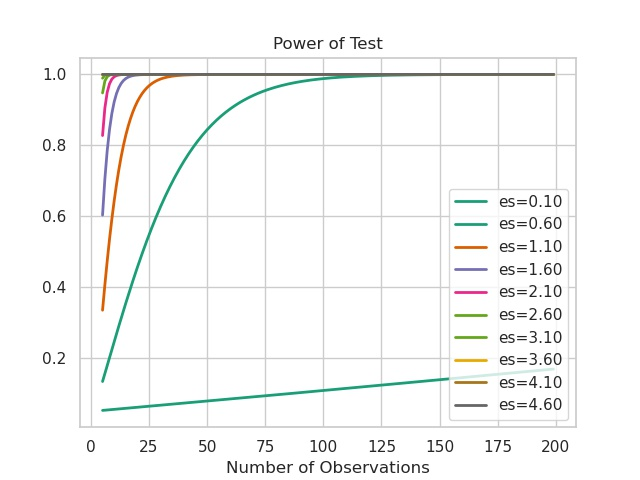
\includegraphics[height = 100mm]{../figures/power_analysis}
	\caption{Predicted statistical power based on effect size and sample size}
	\label{fig:power_analysis}
\end{figure}
\end{center}

\section{Conclusions and other considerations}

Learning is a central feature to political psychology. While there is a robust history and future in political psychology to studying the innate, biological factors influencing how individuals engage with politics, examining how the public learn behavior is still an understudied area of research \citep{sapiro_2004}. While I acknowledge that there are emotional and deeply rooted physiological sources of polarization, it does not happen in a vacuum - particularly when an evolutionary goal of social groups with humans is to foster the learning of group norms and differences as a way to reduce cognitive effort for individuals to constantly evaluate threat \citep{sidanius_kurzban_2013}. 

Political polarization is likely learned and can come from political elites. I acknowledge that this theory does not speak to where elites are learning this behavior. Future work should examine whether these behaviors are the result of institutional incentives. This manuscript's argument also does not consider the way in which the public may provide incentives for politicians to engage in a particular set of behaviors or to provide rewards or punishment for behaving a particular way. This manuscript also does not specify at what point during one's life do they learn these behaviors. While it seems reasonable to assume that teens and young adults concurrently learn these norms while their political attitudes crystalize, this is also an open question. By no means is this theory supposed to explain every way in which norms are learned and the ways in which they travel. Instead, it simply presents an argument encouraging scholars consider a fundamental component of social identity theory which is the establishment of group norms. 

To examine this, I propose both an experiment and an observational study in hopes of cleanly identifying the causal mechanism while consecutively providing a clearer picture of how this causal mechanism manifests in the messiness of real social phenomenon. Again, this observational approach is not perfect and is still susceptible a number of threats to causal inference. Namely, there are a number of backdoor paths which remain open without random treatment assignment, reverse causality, and a violation of the stable unit treatment value assumption given that outside of a lab setting we are likely to learn these behaviors from our peers and not just elites.
\newpage
\bibliographystyle{apsr}
\bibliography{/Users/damonroberts/Dropbox/bibliographies/representation/partisanship,/Users/damonroberts/Dropbox/bibliographies/representation/polarization,/Users/damonroberts/Dropbox/bibliographies/representation/knowledge,/Users/damonroberts/Dropbox/bibliographies/representation/elite_cue_taking,/Users/damonroberts/Dropbox/bibliographies/stereotypes/party_stereotypes,/Users/damonroberts/Dropbox/bibliographies/representation/partisan_homophily,/Users/damonroberts/Dropbox/bibliographies/representation/attitudes,/Users/damonroberts/Dropbox/bibliographies/representation/trust,/Users/damonroberts/Dropbox/bibliographies/representation/participation,/Users/damonroberts/Dropbox/bibliographies/institutions/institutional_theories/congress/parties,/Users/damonroberts/Dropbox/bibliographies/representation/vote_choice,/Users/damonroberts/Dropbox/bibliographies/institutions/institutional_theories/congress/policy_outcomes,/Users/damonroberts/Dropbox/bibliographies/institutions/institutional_theories/congress/dysfunction_and_support,/Users/damonroberts/Dropbox/bibliographies/stereotypes/prejudice_discrimmination,/Users/damonroberts/Dropbox/bibliographies/representation/ideology,/Users/damonroberts/Dropbox/bibliographies/representation/deliberation,/Users/damonroberts/Dropbox/bibliographies/methods/causal_inference}
\end{document}
